\chapter{Prior Art in Terrain Generation}

% Chapter \ref{chapter:DrillOperator} of this thesis introduced a method of describing the surface of the terrain through a series of mathematical operations on the terrain's surface, mimicking a drilling process. Creating this representation required an understanding of terrain surface and a method for mimicking its shape and formation through its inherent mathematical properties. Now that these topics have been explored, the 
Various characteristics of the terrain surface have been quantified and explored in this thesis.
The next step is to use the idea of hydraulic erosion to explore the process of generating terrain data for use in other applications, and study the underlying mathematics of this generation process.

% \section{Why Is Terrain Generation Important?}

Many applications require the generation of, or manipulation of, terrain surfaces, including level design in gaming, world modeling in animation, and terrain compression to name a few. Terrain generation procedures range from randomly perturbing fractals to realistic-looking terrain generation using erosion simulations. Some applications require interactive speed so the user does not need to wait long for terrains to be created, such as in video game applications. Other applications, such as those involving detailed generation simulations for the purpose of modeling or studying the surface, rely more on accuracy and so can sacrifice computation time. 

\section{Fundamental Terrain Generation}

One of the primary methods for generating terrain datasets from scratch is through fractal generation. In the most basic form of fractal generation on a height field, a plateau's center point is set to the average of its corner elevations and then randomly perturbed based on some weighting rules.The terrain is then divided into quadrants and the process is repeated, where each of the quadrant's center points' elevations are set to the average of the corner points' elevations and then it is randomly perturbed \cite{Perlin:1985:IS:325165.325247}. This process is repeated until each pixel's elevation value is set. This process of fractal noise generation is used in many other methods as well \cite{Smelik09asurvey}. 

Fractal modifications on terrains have also been studied. Stachniak and Stuezlinger \cite{Stachniak_Stuerzlinger_2005} present a method for generation of fractal terrains that doubles as a compression scheme for deformed terrains. The method begins with the original terrain and a list of constraints (in the form of a fitness function). The algorithm uses a detailed search algorithm to determine which pixels fail to improve the overall fitness of the terrain, and remove them from the representation. They store the remaining pixels and the original terrain, thus compressing the fractal deformation of the terrain.

Genetic algorithms are also popular methods for terrain generation. Ong et al. \cite{Ong:2005:TGU:1068009.1068241} present a method for random terrain generation which takes as input a polygonal silhouette of a terrain (areas with predefined terrain types) and uses genetic algorithms to randomize the boundaries of the polygonal areas (with constraints). Then, once the areas are well-defined, each is filled in with terrain from a database based on the designated terrain type, and then more genetic algorithms are applied to mutate the terrain to user specifications. 
% 
Walsh and Gade \cite{5585913} present an interactive genetic algorithm where the user inputs a series of parameters and the system generates 8 random terrains based on the parameters (which include cloud cover, lake level, spikiness, etc.). The user then selects their 3 favorite terrains (after a nice graphics engine generates images for them, the "phenotypes"), and these are used as a judge for fitness. Then, two parameters are chosen as parents, offspring are created based on genetic algorithm mutation rules, and new terrains are generated, and the process is repeated until the user is happy.
% 
Frade et al. \cite{FradeVC09} provide a very similar algorithm in that it takes user input (the user chooses the ones he likes the most) and then performs genetic algorithms on the choices to develop new terrains. There are a few primitives used, including a cliff face, sphere, and mountain.

% \subsection{Terrain Generation in Computer Graphics}

Doran and Parberry \cite{Doran2010Terrain} present a technique used for fast terrain generation for games. The algorithm works through agents, who are autonomous and can see and manipulate elevations across the terrain at any point in time. There are five different kinds of agents: coastline, smoothing, beach, river, and mountain. They work in conjunction, but autonomously based on user defined parameters, including how many actions each one takes.

\section{Modeling Hydraulic Erosion}

Chapter \ref{chapter:Introduction} spoke to the importance of hydraulic erosion with regard to the generation of terrain. This theme was once again discussed in Section \ref{section:ChannelNetworkExtraction}, which discussed labeling the pixels of the hydrography network as the most important of the terrain. It is clear that, in order to accurately generate terrain surfaces, erosion must be modeled.

Related works in erosion literature can be divided into two groups, both of which can fall under the heading of Geographic Information Science. Many mathematical models for erosion have been presented in the field of Civil Engineering, for the purpose of studying and predicting the erosion of soil during design and construction of earthen embankments, dams, and levees. Conversely, in the field of Computer Graphics there have been several attempts to simulate hydraulic erosion processes for the purpose of producing more realistic-looking terrains. These erosion simulations, while they do generate realistic terrains, do not model erosion, sediment transport, and deposition with real physical accuracy, and very few authors have attempted to validate their results in any way.

\subsection{Mathematical Erosion Models}

Attempts to explain and model hydraulic erosion processes have been many in the field of Civil Engineering. Some engineers have performed experiments to try to represent in a single quantitative value how susceptible a soil is to erosion, or a soil's \textit{erodibility}. Full mathematical models have also been developed to predict the behavior of earthen levees and dams under erosion conditions. These models are often based on specific geometry of the soil, such as overhangs, head-cuts, and dam breaches. There have also been models developed that describe global ecosystem behavior, incorporating erosion due to its importance in the water cycle and habitat formation, thus defining a landscape's evolution.

% \subsubsection{Landscape and Ecosystem Evolution Models}

Simms \cite{Simms-TortoisesAndHares} gives a brief technical description of the various processes that effect limestone and silicate, two representatives of softer and harder rock types, respectively. He describes erosion
% , or the physical breakdown of rock and soil, 
due to high velocity water, and the threshold of the velocity required before erosion begins. He briefly speaks of hydraulic conductivity and the role it plays on the rate of the rock's erosion. The second process he discusses is dissolution, or the chemical breakdown of rock and soil. This process occurs mainly in softer rocks, but once a threshold velocity of water is reached it can also occur in harder ones. Erosion is dependent upon several soil parameters, including the important hydraulic conductivity. Measurement of these parameters is essential for any erosion simulation to achieve physical accuracy.
% 
Simms' work describes general principles that govern erosion. Beyond this, there are several systems that model erosion on a grander scale, taking into account several different aspects of terrain. Several of these models work on global or macro scales, and although are not immediately applicable for my research, can lend insight into erosion on a smaller scale.

% \subsubsection{IBIS}

Foley et al. \cite{Foley-IntegratedBiosphere} introduce the Integrated BIosphere Simulator (IBIS) land surface model. The IBIS model contains four modules arranged in a hierarchical framework, each dealing with a separate component of the biosphere. The four modules are the land surface, the carbon balance, the vegetation dynamics, and the vegetation phenology modules. Each module of the model works on its own separate time step, which allows the authors to adjust each one individually. The model acts as a series of coupled state machines that interact at different time steps and update each other accordingly.
% 
% The land surface module is broken up into 2 vegetation layers (canopy and ground) and six soil layers (different soil depths). The vegetation layers deal with things such as evaporation and the water cycle. The soil layers deal with the concentration and level of water, ice, etc. This module runs on a 60 minute time step. Then, the second module is the vegetation phenology module, which deals with seasonal changes to the appearance of trees and other vegetation, affecting the levels of evaporation, as well as other processes. This module runs on a 1 day time step. The third module is the carbon balance module, which simply sums all of the photosynthesis calculated in the land surface module and adjusts the carbon level and location. Each of nine different plant function types have their own contributions to the carbon level. This module runs on a 1 year time step. The final module is the vegetation dynamics module, which takes input from all of the other modules and simulates time dependent changes in vegetation cover resulting from adjustments in the other levels from the other modules. This module runs on a 1 year time step.
% 
Delire and Foley \cite{Delire-EvaluatingPerformance} evaluate the IBIS model by comparing a simulation using IBIS to case studies performed for five sites: a soy bean field, a tall grass prairie, a meadow in the Netherlands, a grassland next to a water balance research site, and a forest, all of which are on a significantly larger scale than the simulation requires. 
% They run a set of statistical analyses, plotting their calculated parameter values against the observed values, and checking their mark's distance to the line $X = Y$. This paper demonstrates the necessity for validation, as the IBIS model is extensive, providing little to no intuition that it is correct without data to support it. This validation is further discussed in \ref{section:model_validation}.
% 
Gerten et al. \cite{Dieter-TerrestrialVegetation} present an extension to IBIS. Provided are additions which include an extension of the soil model, with more layers, that includes snow and ice, an extended canopy physiology with two canopies, one of shrubs and one of trees, and extended vegetation dynamics.

% \subsubsection{PALMS}

 Moiling et al. \cite{Moiling-DistributedRunoff} introduce the PALMS landscape modeling system. The authors model the landscape as a grid, and each grid cell contains many inter-connected soil layers that interact with one another, a system that uses the IBIS model described above. Two major factors in the evolution of the landscape are rainfall and runoff, and so the authors also present an erosion model. The model takes into account surface roughness, depression storage, tillage, water and heat transport within the soil, how that effects drainage, etc. Also, the model takes into account how much water is below ground and in what layers this water rests, and where the ground water travels. 
% There are also, taken from IBIS, vegetation and canopy processes, that even go as far as to randomly select where a drop of rain will fall and if it is sits in the canopy or falls down to the earth. The canopy knows how much water rests on the leaves' surfaces, which can evaporate or fall back to earth.
% 
% PALMS is used to detect landscape changes due to erosion. The model is used to measure, over a long period of time, the change in a landscape that is covered in vegetation. For results, the authors chose several areas around the country with known rainfall and landscape data, and used PALMS to accurately predict the changes that occurred to the landscape. 
Bonilla, et al. \cite{Bonilla-TestingGridBasedSoil}  extend the PALMS model to include a more detailed erosion model and wave simulator, as well as taking into account more soil parameters than the original model, such as hydraulic conductivity. 
% The new PALMS model is validated using several vegetation fields with small elevation change in Wisconsin, and it works well for larger data sets. The data was generally on a 5 meter by 5 meter scale, closer to our scale. This data validation is further discussed in \ref{section:model_validation}.

% Both the IBIS model and the PALMS model were designed for use with ecological and agricultural studies. They each incorporate erosion models for the purpose of modeling global phenomena. Both of these incorporated erosion models are too global to use in an erosion simulation to the scale our work requires, while the global models are more complex than is necessary for the simulation. For instance, the IBIS model uses time steps from days to years, whereas our small scale erosion simulation has a time step on the scale of fractions of a second. In contrast, the PALMS model uses a distance scale on the order of a few meters, whereas our work requires tens of meters by tens of meters to model the erosion on a levee. However, it is important to understand that in these works erosion models are being used to solve a larger global problem, in similar fashion to what we proposed.

% \subsubsection{Erosion Models for Overtopping}

In addition to macro scale erosion simulations, in which the total erosion for an entire geographic area is modeled, there have been many erosion models developed for small scale calculations of earthen embankments. These models often calculate the total soil loss or the geometric change of an embankment due to water running over it, often as a result of overtopping. Because the simulator deals with rills and gullies formed on a micro scale and uses them to simulate the total erosion process, these models are often more closely related to this work.

Hanson, et al. \cite{Hanson-PhysicalModeling} conduct seven overtopping erosion tests on large-scale physical cohesive embankment models. The authors test three soil types, two sand and one clay. From the tests, the authors determine a four-stage erosion process that occurs during overtopping of an embankment. In the first stage, flow initiates, causing sheet and rill erosion. One or more ''master rill'' forms, developing a head-cut, thus ending this stage. In the second stage, the head-cut migrates upstream along the embankment, and the stage ends when the head-cut reaches the upstream crest. In the third stage, the crest of the embankment erodes away vertically, culminating when the vertical erosion has ceased. During the fourth and final stage, the breach formed by the eroded head-cut widens, ending when either the water flow stops or the embankment has been completely lost. The observations in this work are intended to be applied and compared to other erosion research done on earthen embankments, and the authors supply data regarding time frames for each stage. Being provided an expected behavior for an embankment under overtopping allows us to validate the erosion simulator on a macro-scale. 

Wang and Kahawita \cite{Wang-ModelingTheHydraulics} present a two-dimensional model of erosion of the profile of an earthen embankment during overtopping. The mathematical model presented was compared to two known case studies, with good results. Their test cases vary in scale from a vertical wall retaining 10 meters of water that suddenly disappears, allowing the water to flow over the terrain, to the Teton Dam failure in 1976, in which 300 million cubic meters of water was allowed to rush over the terrain. In both cases, the results of their model mimic those of the known test case (Teton Dam), and mimic expected behavior of the unknown test case (vertical wall). Similarly, Wang, et al. \cite{Wang-EmbankmentOvertopping} present a two dimensional mathematical model for the erosion of an embankment and compare it to test cases, thereby demonstrating its accuracy. This method is also limited by its dimensionality and its lack of controlled test cases. Due to their limitations, these erosion models are not easily adapted to a more complex data representation of soil, such as layered height fields or the Segmented Height Field representation. Neither of these models are extended to 3 dimensions, allowing for full terrain erosion, because of the complexity introduced by the extension to higher dimensions. 

\subsection{\emph{Erodibility} of Soil}
\label{section:SoilErodibility}

One of the more common modeling techniques involves measuring the \emph{erodibility} of the soil in question. Using this value, the sediment to be eroded is calculated using the velocity of the water that flows over its surface. This calculation provides a quantity of sediment that is picked up by the flow of water to be deposited elsewhere, and can be used as an erosion model for simulation purposes.

Any erosion simulation will require the input of the soil's parameters, and so a method for their measurements is essential. Hydraulic Conductivity of soil is an important parameter needed for many \emph{erodibility} calculations and tests. Unfortunately, this is often one of the hardest soil parameters to measure. Rawls, et al. \cite{Rawls-EstimatingHydraulics} present a series of measurements that allow for the estimation of a soil's hydraulic conductivity. The authors determine correlations between a soil's water retention (in and of itself a difficult parameter to determine, though the authors present a way to do so) and its hydraulic conductivity. This correlation is useful, assuming one can first attain the other measurements necessary to estimate it. Also, this correlation was found through regression-curve fitting, and as such is just an estimation, and probably varies for different types of soils. As is the case with most soil tests, these assume that the soil is heterogeneous, or at least that the soil's water retention is heterogeneous, which may or may not be the case, and often is not.

% \fbox{MAKE A NEW DIAGRAM FOR JET INDEX}
% \begin{figure*}[t]
% 	\centering
% 	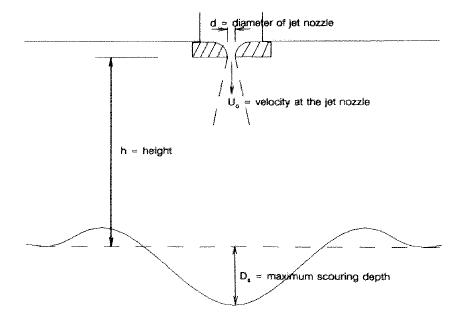
\includegraphics{images/JetIndex.jpeg} \\
% 	\caption[The Jet Index erosion test]{A diagram of the setup of the Jet Index test, showing variables. The jet fires water down on to the terrain, and the rate at which the soil erodes is measured.}
% 	\label{figure:jet_index}
% \end{figure*}

Hanson \cite{Hanson-JetIndex} attempts to tie many standard erosion formulas together with the development of the ``Jet Index''. The author presents a method for measuring a soil's jet index in which a jet of water is buried under the soil in question, and the rate at which the soil is eroded is measured.
% (Figure \ref{figure:jet_index}). 
This measurement is then converted from a jet index value into the soil's ``erodibility'' using well-known empirical formulas, thus tying together a particular measured result with an erosion quantity. In his work, Hanson defines the erodibility of several soil types using this method.

This work demonstrates one of the first attempts to tie empirical formulas for erosion and its various parameters to a single value that can be applied to a soil. The downside to this particular method is the need to measure the jet index of the soil, unless a pretested soil is used. Due to the vastly heterogeneous nature of soil, two soil samples will almost certainly have different jet indexes, despite how similar their compositions may be. This can be rectified somewhat by performing many tests on similar soils and applying an ''erodibility'' to a soil classification instead of a particular soil, though this method can be time-consuming and expensive. And so this measurement for erodibility is often not practical for computer simulation.

Annandale \cite{Annandale-Erodibility} links several soil parameters and how they affect the energy gained or lost by the soil when a jet of water is run over it together through a series of tests. He looks at the relationships between these parameters and defines a new, single measurement that he refers to as a soil's \emph{Erodibility Index}.  This measurement is based on the correlation between the rate of energy dissipation of the flow of water and previously observed behavior of the earth mass erodibility of soil.

Similar to Hanson's Jet Index work described above, this method requires a measurement of erosion for a particular soil in order to be useful. However, unlike Hanson's paper, he develops equations for a soil's erodibility based on other known (measurable) parameters of the soil. Assigning a single empirical value to a soil based on the soil's measurable parameters allows for a useful erosion model, assuming that the parameters of the soil are readily measurable or accessible.

Temple and Moore \cite{Temple-HeadcutAdvance} model the erosion of head-cuts in earthen spillways. A head-cut is a sharp drop off in the slope of an incline, thereby creating a channel for water falls. The authors divide the erosion of a head-cut into three separate phases and model each independently. They also define a new parameter, the ''Head-cut Erodibility Index'', which quantifies the tendency for the soil int he spillway to erode into a head-cut. They also use the flow energy dissipation rate, as Annandale, to model the rate at which the top of the head-cut erodes away.

Additionally, Moore \cite{Moore-FieldProcedures} describes the field procedures necessary to measure the various parameters needed to calculate the Head-cut Erodibility Index described by Temple and Moore \cite{Temple-HeadcutAdvance}. By giving a more basic mathematical definition of the index, Moore simplifies the calculation to obtaining a series of four parameters, and provides methods to determine each one. With both of these papers, the authors seek to unify all erosion processes that occur to form head-cuts into a single parameters that can be easily measured, and provide methods for doing so.

This model, while a step forward, is limited to the erosion of a particular geometric shape, defying the generality that is needed for accurate simulation. An ideal erosion simulation will maintain its coherence regardless of whatever shape the levees take during it, without the need for specific erosion models for each shape classification, such as a head-cut. However, these models may be useful in determining when the levee has reached a particular shape, thus helping to identify good or poor design, and how to improve upon it.

% \subsubsection{Erodibility Tests}

Many authors have developed tests to measure the rate of erosion of a particular soil type. These tests usually involve the design and development of new devices that measure the rate or erosion of a soil, a step forward from the ''jet index'' measurement by Hanson \cite{Hanson-JetIndex}.

One version of an erodibility test is presented by Brandimarte, et al. \cite{Brandimarte-StochasticFlow}, in which they present a simulation method for determining the likelihood of reaching the critical scour depth, or the amount of soil that is eroded away from the columns of a bridge before the bridge collapses. The authors' method is run many times in a Monte Carlo fashion in order to determine the chance that the bridge will fail in a certain length of time. Although not directly measuring a soil's erodibility, the method does use the soil's parameters to calculate, or estimate, the rate of erosion of a soil, which is the same information the soil's erodibility would provide. This method for probabilistically determining the chance of failure of a structure is useful in validating erosion simulations by providing another error metric for the simulation's results.

Wan and Fell \cite{Wan-InvestigationOfErosionRate} describe the development of two new erosion rate tests, known as the Hole Erosion Test (HET) and the Soil Erosion Test (SET). Both presented tests require elaborate apparatuses to measure the rate of erosion. Once again, however, the authors attempt to tie the soil parameters measured with their instruments to the soil's erodibility.

The authors also go to great lengths to describe that practical applicability of their measurements. They first discuss a correlation between their measurements and the soil's erodibility, and then use this correlation to describe methods to predict the erodibility index from various soil parameters that are already well known. The authors model the correlation through a series of linear equations, some of which contain parameters that are difficult if not impossible to measure, and so must be estimated. The authors stress, however, that the actual tests should be used whenever possible, as they exhibit a higher degree of accuracy than the equations.

Finally, the authors present a method assessing the likelihood of internal erosion and piping of an embankment dam, a process that is central to the levee erosion problem. Their assessment is useful in the later portions of an erosion model, during which a pipe may expand to the size necessary to breach a dam or embankment.

While these tests, and all measurements of a soil's ''erodibility,'' demonstrate a knowledge about a specific soil type and are overall the most useful tools in studying the erosion of levees, they lack the practicality necessary to be able to plug their results into an erosion simulation run on a computer. 
% For this reason, we turn to another correlation between a measurable value and the erodibility of a soil.

% \subsubsection{The Erodibility Index}

Briaud's work in New Orleans after Hurricane Katrina is based heavily on his own definition of a soil's erodibility. In his work, he strays from a traditional definition of a soil's erodibility, the ratio between the soil's rate of erosion ($\dot{Z}$) and the velocity of the water causing the erosion. Because water velocity varies through the flow field and the velocity at the soil-water interface is technically 0, an accurate single value for the erodibility of soil based on the previous definition is not plausible. Instead, erodibility is treated as a function that is based on the hydraulic shear stress, or pull of the water on the soil, changing with water velocity so that it can be defined along the water/soil boundary.

A soil's erodibility, as Briaud defines it, is a function of the shear stress ($\tau$) of the soil at the soil/water interface. This definition incorporates the geometry of the soil as well as the water's properties along the flow field. Its definition is expressed in the following equation:

\begin{align}
	\dot{Z} = f\left(\tau\right)
\end{align}

Here, $f\left(\tau\right)$ is based on the shear stress, the critical shear stress, velocity and density of the water, and various soil parameters. This definition allows for erodibility to be defined over the entire water/soil boundary. 

Because Briaud's definition of erodibility is expressed as a function of shear stress and erosion rate, tests were required to characterize the relationship between the two properties. To conduct these tests, Briaud assembled an apparatus in which he allowed water to flow through packed dirt, measuring the rate of erosion, while controlling the shear stress. With these data, he created a correlation between the properties and proposed a series of erosion categories into which soils fit based on their parameters \cite{Briaud-ErosionByOvertopping}. He advises that those soils that fall toward the categories of ''highly erodible'' should be avoided when creating levees or dams to control the flow of water. A highly erodible soil, such as sand, erodes at a rate on the order of more than 100 mm per hour when contacting any running water at all. Soils that require the water to run at a velocity of at least 1 meter per second fit into a slightly less erodible category. A soil has medium erodibility if it is eroded 1 mm per hour by water rushing at 1 meter per second. Many soils fall around this value. Some of the least erodible soils, according to Briaud, erode at a rate of approximately 5 mm per hour when being eroded by water traveling at 7 meters per second.

Briaud \cite{Briaud-CaseHistories} describes four famous structures with failure cases to which he has applied his erodibility function. In each case, he has performed numerical analysis and determined a prediction for the scour depth at which the various geological structures would fail, given the geometry and soil type of the structure and the water velocity data from the time of the structure failure. Given soils data, Briaud calculated the probability of failure of the structure given a certain length of time. Each case history demonstrates a different use for the erodibility function and Briaud's erosion function apparatus. Further discussion of the Hurricane Katrina case history can be found in Section \ref{section:model_validation}.

Briaud's definition of erodibility fits in nicely with this project's research goals, as it creates a function of erodibility applied to a specific type of soil, dependent upon the geometry of the water/soil boundary, which is calculable given the shape of the soil and the velocity of the water flowing over it. This is ideal for a small-scale erosion simulation, in which there are calculations of 
% In our research we will use Briaud's erodibility function to calculate 
the rate of erosion of a specific area of the soil/water boundary, given the soil parameters and the speed and direction of the flow of water, thus determining how much soil is eroded during each time step of the simulation.


\subsection{Erosion Simulations}
\label{section:PriorLiteratureErosionSimulation}

As in civil engineering, a lot of work has been done in computer graphics to simulate erosion, often for the purpose of developing more realistic-looking terrain geometry. As a result of this, research in the community is almost always solely concerned with how ''good'' or realistic the final product looks, and not how physically accurate the simulation is. However, there is little research in the area that involves any sort of physical validation beyond that of simply looking close to the ideal terrain. 

% \subsubsection{Early Terrain Development}

The major force involved with terrain development is hydraulic erosion. Because of this, much research in computer graphics is geared toward simulating erosion on terrains to develop realistic-looking scenes.

Early erosion simulations worried only about the overland flow of water. Musgrave, et al. \cite{Musgrave-SynthesisAndRendering} perform a basic erosion simulation on a height field in which each grid space stored an altitude, a height of water, and a layer of sediment. As water rushed over the grid cell, sediment could either be picked up or deposited, depending upon the total carrying capacity of the water and the height of the water. When the water level reaches below zero, the sediment is deposited. An interesting twist to the algorithm is the use of weathering of the terrain, a different phenomenon altogether from hydraulic erosion.

Kelley, et al. \cite{Kelley-TerrainSimulation} devise a way to produce fractal terrain from forming a stream network and growing the terrain up around it, as if performing a reverse erosion simulation. The terrain is built on a triangle network, along the edges of which the stream may form according to a series of rules. Along similar lines, Prusinkiewicz and Hammel \cite{Hammel-FractalMountainsRivers} present a fractal terrain generator that divides the plane in to triangles. A ''squig curve'', or discretized running curve, is randomly cast along the edges of the triangles throughout the terrain. The neighboring triangles are then bisected and the processes is repeated, adding detail to the curve. At each bisection, each new triangle is given a random elevation jitter. Each of these papers share the idea that terrain should be formed using rivers and hydraulic erosion.

Nagashima \cite{Nagashima-ErodedValleyGeneration} generates terrains by using physically based erosion models to carve out riverbeds in mountainous terrain. This method, like the previous ones discussed, forgoes a fluid simulation approach in favor of a mathematical approach to terrain generation. Early methods avoided a full fluid simulation often because of its high computational complexity.

Li and Moshell \cite{Li-ModelingSoilDynamics} present the Dynamic Terrain system, in which they use an interactive terrain generation system and allow a user to conduct excavation activities (more specifically, erosion by a blade) to alter the shape of the terrain. They calculate the modifications to the soil using the shear stress applied to it. The authors' main concern is whether or not a given soil configuration will fail, and if so under what conditions it does. This was an early attempt to adapt an erosion model to a computer simulation for the purpose of analyzing a specific soil configuration under erosion conditions. As such, it is a key milestone in computer modeling of erosion, but is not convenient for use with a more complex data structure for soil, such as the one used in this research, due to the lack of complexity in the terrain that it allows, such as undercuts or even heterogeneous soils. Also, the model uses the geometry alone to calculate the erosion and weathering of the soil, and although their method may be extended to hydraulic erosion it is not immediately clear what form this extension would take.

Later attempts at terrain generation, such as Chiba et al. \cite{Chiba-VelocityFields}, incorporate erosion simulation involving fluid simulation to carry sediment downstream. The authors divide the terrain into a grid-based velocity field, over which they track the direction of speed of water flowing over it. The fluid model is simplistic, assuming that the fluid flows in the direction of steepest gradient without any emphasis put on the pressure or volume of the fluid.

More recently, Wang, et al. \cite{Wang-ErosionProtection} present the results of a project that allows the user to dynamically change terrain data on which an erosion simulation may be run. The purpose of the project is to allow civil engineers to visualize the effect of erosion on various terrain configurations. This is an early coupling between civil engineering and computer graphics, and mirrors this project's overarching goals.

% \subsubsection{Physically-Based Erosion Simulation}

% Beyond terrain generation, research in computer graphics has also focused on erosion for the purpose of animation. Efficient algorithms that can be updated and changed dynamically are essential for erosion simulations.
% 
% \subsubsection{Terrain Modeling}
% 
% Several applications of computer graphics, including computer generated images and video games, require realistic-looking terrains. Therefore, many erosion simulations have been implemented for the purpose of developing these terrains. Because hydraulic erosion is the most important process in shaping terrains, most terrain development is done by either simulating erosion or mimicking it. In 1988, in \cite{Kelley-TerrainSimulation}, Kelley et al., build a stream network along a discretized terrain, simulating river flow. By assigning flow values to the nodes in their stream network tree, they simulate the flow of streams through the terrain. Following a series of rules, they develop the terrain up around the stream network, first deciding where the source and the sink are and then what the terrain would look like if it had been carved out by the modeled stream network. 
% 
% Musgrave et al. \cite{Musgrave-SynthesisAndRendering} first model a terrain with fractal terrain generation and Perlin noise, and then cast rain over the surface, running a simple erosion simulation where the water in a grid space runs to its lowest neighbor, picking up sediment as it goes and depositing it when the water height in a cell reaches zero. The simulation also accounts for weathering, and soil can tumble down if the slope between grid spaces is too steep. The simulation is designed to add detail to an already-established terrain.
% 
% Nagashima \cite{Nagashima-ErodedValleyGeneration} uses an erosion model on a terrain to calculate the erosion process along the grid. The method, for the most part, ignores the nuance of the geometry of the system as a whole, and results in terrains that are fundamentally realistic but are limited by the scope of the equations used, because they only apply to fast-moving rivers that carve out the terrain. The method also ignores fluid dynamics, relying on basic rules of fluid movement and the erosion model to produce results. However, it is an important method in that it is one of the first to use erosion models from civil engineering in a computer erosion simulation.
% 
% The next step in terrain generation was taken by Chiba et al. \cite{Chiba-VelocityFields}. The authors used a velocity field spread across a terrain to keep track of the flow of water, and coupled this with known sediment erosion equations calculate how much sediment would be either deposited (from incoming flow) or eroded (from outgoing flow) at each grid space. The velocity field is complex and close to a full fluid simulation, if only in two dimensions. This method brings together a simple fluid simulation with terrain and erosion modeling.

% \subsubsection{Erosion Simulation}

In recent years, erosion simulation has developed in to an area of computer graphics that relies heavily on work in the field of engineering. Since the early papers of the late 1990s, erosion simulation has included fluid simulation and complex terrain modeling based on work done in the field of soil sciences.

In an early attempt the simulate weathering processes for the purpose of changing the appearance of the underlying structure, Dorsey et al., in \cite{Dorsey-FlowAndChanges} use particle hydrodynamics to simulate the flow of water over a volumetric model, allowing the water particles to pick up and later deposit sediment from the surface, thus eroding and repositioning portions of the volume. The absorption model used in the work is based on the properties of the surface, including porosity and absorptivity. The model also simulates staining by dissolving materials from one portion of a water's flow and depositing them elsewhere, thus creating layers of different materials. Thinner layers on top of thicker layers can cause staining. In this model, deposition occurs when the amount of sediment that is being carried by a water particle exceeds the particle's limit, and thus it ''drops'' sediment. Absorption can also remove material from the top layer of a stain, thus removing the stain. For a fluid simulation, a velocity map is used, and the surfaces are modeled by volumetric models. As opposed to several other erosion simulation attempts in the 1990s, this method tracks particles over a volumetric model, abandoning a grid entirely. This erosion model was used mainly for texture mapping staining effects and not volumetric carving. The erosion performed was limited in scope because of the materials being used and the overall goal. The volumes were not eroded but instead slightly weathered, giving them a worn look.
% , but this method is ultimately not what we need.

Neidhold et al. \cite{Neidhold-Interactive} present an erosion simulation that coupled a terrain with a particle fluid simulator. The terrain is represented by a variation on a layered height field, where each grid space contains five layers representing different data layers: 3D acceleration, 3D velocity, fluid level, dissolved material, and soil height. Finite difference algorithms are applied between neighboring layers, which allow the erosion simulation to adjust each layer according to various rules. For the fluid simulation, the authors use Navier-Stokes equations, which in turn update the level of the fluid in each grid space. With updated velocity and acceleration, the authors are able to calculate how much soil is absorbed in to the water, updating the sediment and soil height layers. When a grid cell's fluid's carrying capacity is exceeded, sediment is deposited, adjusting the lower layers. While this method is fast on a 256 by 256 terrain, it does not deal well with complex terrains, such as cliffs (although no specific slope limit was provided), and cannot handle undercuts or overhangs, or even heterogeneous soils.

Benes has published much work in computer graphics in the area of hydraulic erosion simulation. He and Forsbach \cite{Benes-SimulationHydraulicErosion} present a fairly simple but powerful erosion simulation technique. Using Benes's layered heightfield \cite{Benes-LayeredDataRep} the authors present an erosion model on a terrain grid that involve a series of equations that govern sediment transport, erosion, and deposition. Water is modeled as a layer in the layered height field, and during the first step of the simulation water flows from areas of higher altitude to areas of lower altitude in an attempt to balance the water level over the terrain. Water can pick up sediment as it travels over the surface according to a series of parameters and equations. Their technique does not allow for complex terrain surfaces. The fluid flow is a shallow-water simulation in which all water in a grid cell flows the same direction, not allowing for more complex fluid flow patterns, and as such is not ideal for modeling detailed erosion processes.

Benes, et al. \cite{Benes-HydraulicErosion} present a method for simulating hydraulic erosion on a homogeneous terrain. The terrain is modeled as a voxel grid where each cell in the grid has a state associated with it. The cell is either water, air, or soil. As water flows, the cells can transition from soil to water (with sediment) and back, making the sedimentation process fast. The method performs Navier-Stokes with each time step, but focuses on the boundary cells (those that are fluid cells with some sediment). The surface is eroded away or built up by changing the state of the boundary cells, and so the precision of the surface is restricted slightly by the vertical resolution of the voxel grid. Their method has unique processes for the fluid and the fluid-surface interface, and models air as a separate material. It also allows for some soil properties to be taken in to account, such as whether the material is cohesive or cohesionless. However, the lack of heterogeneous terrains, dependence of voxel grid resolution and lack of physical accuracy, and spatial and temporal complexity of the voxel grid lead us away from the voxel method.

Moving in a different direction, Benes \cite{Benes-ShallowWaterSimulation} designs a shallow-water erosion simulation, and instead of continuing to use his layered height field he chose a simple two layer field, where there is a layer of water above a homogeneous layer of soil. During the course of the simulation, a third layer of sediment, or regolith, forms between the water and the soil. The water flow is calculated using two-dimensional Navier-Stokes equations, which use a separate time step from the erosion simulation. The main purpose of this simulation is to present erosion in real time, and such there are many shortcuts taken to reduce time complexity, starting with the use of a two-dimensional height field for both the fluid and the terrain representation. 
% Because time is not as much of an issue for our work, we will use a complex representation and algorithm for our erosion simulation.

Most recently, Kristof and Benes, et al. \cite{Benes-SmoothedParticles} present an erosion simulation using Smoothed Particle Hydrodynamics (SPH). The soil, water, and soil-water boundary are all represented by particles, the soil and water particles have mass and velocity while the boundary particles are designed solely for the two phases to interact. The fluid particles flow according to adjusted Navier-Stokes equations, The authors also create special boundary particles that act as an interface between the fluid and the soil particles. In the simulation, boundary particles are spread along the soil surface and whenever some are absorbed by the passing water the level of the soil is adjusted, and new particles are created on the boundary to replace the missing ones. This method allows for the soil, the boundary, and the fluid to all have different parameters that interact with those of the other states without the need to adjust the resolution or time step. Representing both the fluid and the soil as particles also allows for sediment transport between fluid particles. Boundary particles can draw soil particles out of the water, which simulates deposition, or the water can draw soil particles from the boundary, which simulates sedimentation. In this method, the soil is stored as a heightfield, and each grid cell translates in to a different number of soil particles. This method can handle more complex terrains than Benes's previous work, but still is limited by the shape of the terrain and the use of a height field to represent it, so it does not support overhangs. However, this method is meshless, avoiding terrain and fluid surface artifacts that arise from the rigidity of a grid-based representation like a height field. Also, the fluid simulation and the accuracy of the terrain heights are not restricted by resolution, as is the case with voxel grids.

\section{Validation}

% One of the major goals of this project is to present an erosion simulation that has been validated by physical experimentation.

\subsection{Erosion Model Validation}
\label{section:model_validation}

Many of the erosion models discussed above have provided case study validation. For the IBIS model, comparison testing was performed on the five test sites mentioned above. For each test case, statistical analysis was performed, including root mean square error (RMSE) and mean biases for parameters such as soil moisture content, snow depth, and total monthly runoff. Except for a few outliers, the data confirms IBIS's usefulness as an ecological system simulation based on their error metrics, especially considering that the data was taken for large ecological sites, such as a Russian grassland. For the PALMS model, validation was performed on three different farms in Wisconsin, all using 2 years' worth of data. The data was broken down in to individual runoff events (rain storms, for example) and each event was analyzed separately. For each event, calculated soil loss was compared to observed soil loss, and the coefficient of determination, RMSE, and model efficiency values were computed. For PALMS, the RMSE was as low as 1 mm for most data (the rainfall depth was generally greater than 12.7 mm, or $\frac{1}{2}$ an inch). 
% This kind of analysis is a step towards what we will perform on our simulation, comparing soil loss values for specific runoff events.

Many of the other erosion models that were mentioned previously have provided some degree of validation to confirm their accuracy. Wang and Kahawita \cite{Wang-ModelingTheHydraulics} compare their results to two test cases, one fictitious and one based on an actual flooding event. Wang et al. \cite{Wang-EmbankmentOvertopping} use their terrain software to simulate the Supa River basin, a 70.6 km stretch of land that receives about two meters of rainfall a year. They model the waste stations and other objects that line the river bank, but make no statistical comparison to actual erosion in the area.

By definition, all soil erodibility studies were based on both field and laboratory tests, and thus are validated by the methods used to procure them. Briaud \cite{Briaud-CaseHistories} uses his values for soil erodibility for comparison to four case studies, calculating each case's failure probability. In the case of New Orleans's levees during Hurricane Katrina, Briaud was able to use his erodibility model to categorize the soil from many of the levees that failed as ''highly erodible''.

\subsection{Erosion Simulation Validation}
\label{section:sim_validation}

To my knowledge, validation of computer simulations has not yet been accomplished anywhere in the literature, though it has been attempted with some success by the SODA project. Valette et al. \cite{Valette-SoDA} present work in which they take a sample of soil and model it as an extended cellular automaton on a grid, where each cell of the grid has many possible states, ranging from surface to sediment. Rain is randomly applied to the surface, and each surface cell's states is recalculated, allowing some cells to be detached from the surface and travel with the water, a different state of a cell. Deposition and sedimentation are handled via cell state changes.

What is most important about this work is that the authors performed an experiment with the same setup and visually compared the results of their simulation to their experimental results. Visually, it is difficult to tell how accurate their simulation is, because very little of the soil was actually transported and the rain dropped on the soil did not noticeably deform the soil surface. Their statistical analysis consists of determining where the terrains' heights differ, and by highlighting these areas for the reader to see. No quantitative analysis was performed. 
% We wish to extend on this validation to include statistical analysis and a firmer understanding about what it means for an erosion simulation to be physically accurate.



% \section{Generating Terrain Data Using Drill Operator}
% 
% \fbox{Does this work?}


\section{Summary of Prior Art in Erosion Modeling}

There are a multitude of erosion simulations, in both civil engineering and computer graphics literature.
Many of these are limited in their scope, such as those in a 2D system. Others lack physical
accuracy, concerned solely with generating realistic-looking terrains. One common thread through
all of the simulation methods is the lack of statistical validation.

In order to better understand the process of erosion, and therefore better understand
the underlying mathematics of terrain formation and hydrography, a physically accurate
simulation of hydraulic erosion is necessary. With this simulation, small-scale erosion
can be studied through analysis of the formation of channels along the surface, 
velocity and behavior of water, and failure conditions of earthen levees and dams.

Chapter \ref{chapter:ErosionSimulation} presents
such a simulation, including a comparison to laboratory experiments of eroded terrains
for both visual and statistical validation.






